% This file was created by matlab2tikz.
%
%The latest updates can be retrieved from
%  http://www.mathworks.com/matlabcentral/fileexchange/22022-matlab2tikz-matlab2tikz
%where you can also make suggestions and rate matlab2tikz.
%
\definecolor{mycolor1}{rgb}{0.00000,0.44700,0.74100}%
\definecolor{mycolor2}{rgb}{0.85000,0.32500,0.09800}%
%
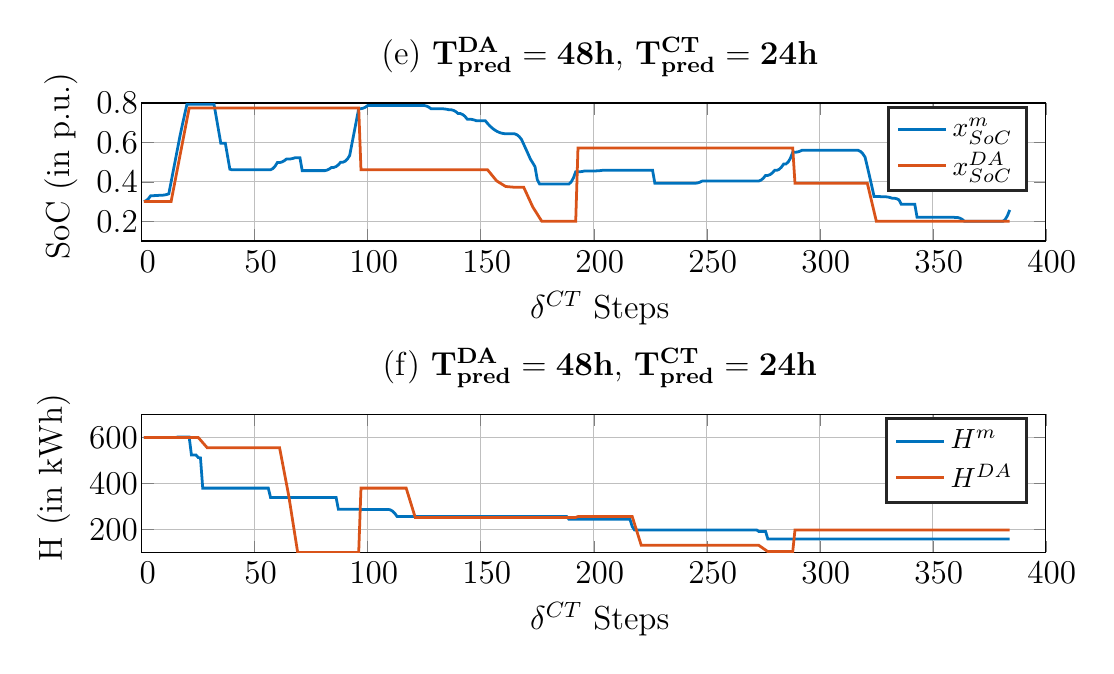
\begin{tikzpicture}

\begin{axis}[%
%width=2.223in,
%height=2.843in,
%at={(1.354in,4.865in)},
width=4.521in,
height=0.69in,
at={(0.758in,3.357in)},
scale only axis,
xmin=0,
xmax=400,
ymin=0.1,
ymax=0.8,
ylabel style={font=\color{white!15!black}},
ylabel={SoC (in p.u.)},
axis background/.style={fill=white},
xmajorgrids,
ymajorgrids,
yticklabel style = {font=\large,xshift=0.5ex},
xticklabel style = {font=\large,xshift=0.5ex},
ylabel style = {font=\large,xshift=0.5ex},
xlabel style = {font=\large,xshift=0.5ex},
ytick scale label code/.code={$\times 10^{#1}$},
/pgf/number format/precision=5,
xlabel={$\delta^{CT}$ Steps},
title style = {font=\large,xshift=0.5ex},
title={(e) $\mathbf{T^{DA}_{pred}=48h,\,T^{CT}_{pred}=24h}$},
legend style={legend cell align=left, align=left, draw=white!15!black, line width=1}
]
\addplot [color=mycolor1, line width=1]
  table[row sep=crcr]{%
1	0.300000000000011\\
2	0.305033743096828\\
3	0.315101229290519\\
4	0.330202458581084\\
5	0.330202458581084\\
6	0.330538620867628\\
7	0.331210945440716\\
8	0.332219432300406\\
9	0.332219432300406\\
10	0.33346850644682\\
11	0.33596665473965\\
12	0.339713877178951\\
17	0.636588877178951\\
18	0.68995847765899\\
19	0.742191942226327\\
20	0.793289270880962\\
32	0.793289270880962\\
35	0.59592084982836\\
37	0.59592084982836\\
39	0.464341902459921\\
40	0.461350128735319\\
57	0.461350128735319\\
58	0.467449260679757\\
59	0.479647524568634\\
60	0.497944920402006\\
61	0.497944920402006\\
62	0.500897931314682\\
63	0.506803953140093\\
64	0.51566298587818\\
65	0.51566298587818\\
66	0.516881210084534\\
67	0.519317658497243\\
68	0.52297233111625\\
70	0.52297233111625\\
71	0.457182857432088\\
81	0.457182857432088\\
82	0.459914390170184\\
83	0.465377455646376\\
84	0.473572053860664\\
85	0.473572053860664\\
86	0.477938472511426\\
87	0.486671309813005\\
88	0.499770565765402\\
89	0.499770565765402\\
90	0.504963333622527\\
91	0.515915838387002\\
92	0.533912098201768\\
96	0.771412098201722\\
97	0.771412098201722\\
98	0.773918435041708\\
99	0.779264619927631\\
100	0.787450652859491\\
125	0.787450652859491\\
126	0.78469212054506\\
127	0.779175055916198\\
128	0.770899458972963\\
133	0.770899458972963\\
134	0.770034828078735\\
135	0.768305566290337\\
136	0.765711673607711\\
137	0.765711673607711\\
138	0.762485481348335\\
139	0.756033096829583\\
140	0.746354520051455\\
141	0.746354520051455\\
142	0.741680901751863\\
143	0.732333665152737\\
144	0.718312810254019\\
145	0.718312810254019\\
146	0.71698053200862\\
147	0.714315975517763\\
148	0.710319140781507\\
152	0.710319140781507\\
153	0.696316278324787\\
154	0.68402933453342\\
155	0.673458309407465\\
156	0.664603202946864\\
157	0.657464015151731\\
158	0.651852795935042\\
159	0.64776954529691\\
160	0.645214263237222\\
161	0.64418694975609\\
162	0.643760853721801\\
165	0.643760853721801\\
166	0.639093463082304\\
167	0.629758681803253\\
168	0.615756509884648\\
169	0.590825368098706\\
170	0.565657971209532\\
171	0.540254319217127\\
172	0.514614412121432\\
173	0.496377385456583\\
174	0.476965470976324\\
175	0.411175997292105\\
176	0.389414307181028\\
189	0.389414307181028\\
190	0.399775056188957\\
191	0.420496554204817\\
192	0.451578801228663\\
194	0.451578801228663\\
195	0.45315752115971\\
196	0.455525601056308\\
198	0.455579038556266\\
201	0.455846226056281\\
202	0.45636976276262\\
203	0.457416836175355\\
204	0.458987446294373\\
226	0.458987446294373\\
227	0.393197972610153\\
245	0.393197972610153\\
246	0.395068567848284\\
247	0.398809758324433\\
248	0.404421544038712\\
273	0.404421544038712\\
274	0.409179837689521\\
275	0.41869642499114\\
276	0.432971305943511\\
277	0.432971305943511\\
278	0.437241687887933\\
279	0.445782451776836\\
280	0.458593597610161\\
281	0.458593597610161\\
282	0.463975328760966\\
283	0.474738791062521\\
284	0.490883984514937\\
285	0.490883984514937\\
286	0.500774634316542\\
287	0.520555933919695\\
288	0.550227883324453\\
289	0.550227883324453\\
290	0.551484158978326\\
291	0.554730434939302\\
292	0.559966711207267\\
317	0.559966711207267\\
318	0.554232912106158\\
319	0.542765313903942\\
320	0.525563916600674\\
321	0.477264423448162\\
322	0.427865473743338\\
323	0.377367067486261\\
324	0.325769204676931\\
325	0.325769204676931\\
326	0.325587259240592\\
327	0.325223368367915\\
328	0.324677532058843\\
329	0.324677532058843\\
330	0.323435801687936\\
331	0.320952340946064\\
332	0.317227149833286\\
333	0.317227149833286\\
334	0.314558234348226\\
335	0.309220403378049\\
336	0.286702856171019\\
342	0.286702856171019\\
343	0.220913382486799\\
359	0.220913382486799\\
360	0.21924091579001\\
361	0.21924091579001\\
362	0.216034096491683\\
363	0.209620457895028\\
364	0.199999999999989\\
381	0.199999999999989\\
382	0.209587837301569\\
383	0.228763511904788\\
384	0.25752702380953\\
};
\addlegendentry{$x^m_{SoC}$}

\addplot [color=mycolor2, line width=1]
  table[row sep=crcr]{%
1	0.300000000000011\\
13	0.300000000000011\\
21	0.774999999999977\\
96	0.774999999999977\\
97	0.461350128735319\\
153	0.461350128735319\\
157	0.405338678908322\\
161	0.376781927727677\\
165	0.372672673803095\\
169	0.372672673803095\\
173	0.272948106659385\\
177	0.199999999999989\\
192	0.199999999999989\\
193	0.572087424662698\\
288	0.572087424662698\\
289	0.393197972610153\\
321	0.393197972610153\\
325	0.199999999999989\\
384	0.199999999999989\\
};
\addlegendentry{$x^{DA}_{SoC}$}

\end{axis}

\begin{axis}[%
%width=2.223in,
%height=2.843in,
%at={(4.279in,4.865in)},
width=4.521in,
height=0.69in,
at={(0.758in,1.8in)},
scale only axis,
xmin=0,
xmax=400,
ymin=100,
ymax=700,
ylabel style={font=\color{white!15!black}},
ylabel={H (in kWh)},
axis background/.style={fill=white},
xmajorgrids,
ymajorgrids,
yticklabel style = {font=\large,xshift=0.5ex},
xticklabel style = {font=\large,xshift=0.5ex},
ylabel style = {font=\large,xshift=0.5ex},
xlabel style = {font=\large,xshift=0.5ex},
ytick scale label code/.code={$\times 10^{#1}$},
/pgf/number format/precision=5,
xlabel={$\delta^{CT}$ Steps},
title style = {font=\large,xshift=0.5ex},
title={(f) $\mathbf{T^{DA}_{pred}=48h,\,T^{CT}_{pred}=24h}$},
legend style={legend cell align=left, align=left, draw=white!15!black, line width=1}
]
\addplot [color=mycolor1, line width=1]
  table[row sep=crcr]{%
1	600\\
15	600\\
16	601.749382661229\\
21	601.749382661229\\
22	523.967158067371\\
24	523.967158067371\\
25	512.701890665498\\
26	510.886107432959\\
27	379.630919480866\\
56	379.630919480866\\
57	338.868438750402\\
86	338.868438750402\\
87	287.878281036659\\
96	287.878281036659\\
97	287.137145023378\\
109	287.137145023378\\
110	285.173134588183\\
111	279.318160083261\\
112	269.572221508614\\
113	255.935318864241\\
188	255.935318864441\\
189	244.077142651942\\
216	244.07714265201\\
217	212.801202891545\\
218	197.967134915961\\
272	197.967134915961\\
273	191.148683593775\\
276	191.148683593775\\
277	158.497077806576\\
384	158.497077806886\\
};
\addlegendentry{$H^m$}

\addplot [color=mycolor2, line width=1]
  table[row sep=crcr]{%
1	600\\
25	600\\
29	554.938930392506\\
61	554.938930392506\\
65	349.199573105657\\
69	100\\
96	100\\
97	379.630919480893\\
117	379.630919480893\\
121	252.377564330606\\
192	252.377564330606\\
193	255.935318864481\\
217	255.935318864481\\
221	130.831559822621\\
273	130.831559822621\\
277	103.557754533875\\
288	103.557754533875\\
289	197.967134915961\\
384	197.967134915961\\
};
\addlegendentry{$H^{DA}$}

\end{axis}
\end{tikzpicture}%